\chapter{Wstęp}
\label{cha:introduction}
Założeniem projektu, było stworzenie modułu sensora, zgodnego ze standardem mikroBUS\texttrademark. Korzystając z okazji na zdobycie nowych umiejętności, zdecydowano się rozszerzyć założenia projektowe o dwa dodatkowe sensory (co daje łącznie trzy układy pomiarowe na jednej płytce). Układy te, komunikują się z mikroprocesorem STM32F103 znajdującym się na tej samej płyce. W procesorze, dane są przetwarzane, nakładając dodatkową warstwę abstrakcji dla obsługi sensorów. Z płytką, można komunikować się przy użyciu interfejsu UART. Dodatkowym założeniem projektu, było różne podejście do tworzenia oprogramowania, każdego z członków zespołu. Zdecydowano, że jeden z członków zespołu będzie tworzyć kod, testując go z mikroprocesorem STM32F4, kolejny bezpośrednio na wykonanej płyce, a ostatni bez bezpośredniej styczności ze sprzętem. Podejście to, pozwoliło spojrzeć na pojekt z innej perspektywy, jak gdyby zespół był większy i rozproszony. Cały proces tworzenia był kontrolowany przy użyciu platformy Github, pozwalającej na wygodną kontrolę wersji oraz dyskusję nad kolejnymi zmianami w kodzie. \newline\newline
W niniejszym sprawozdaniu, skupiono się przede wszystkim na procesie tworzenia modułu oraz popełnionych błędach, nie pomijając krótkiego wstępu teoretycznego. Całość, zakończona jest wnioskami na temat procesu oraz zdobytych umiejętności.
\section{Podsumowanie założeń}
\begin{itemize}
    \item Zaprojektowanie płytki z mikroprocesorem i konwerterem UART-USB
    \item Diody LED sygnalizujące stan układu
    \item Wyprowadzenia zgodne z mikroBUS\texttrademark
    \item Trzy czujniki na jednej płytce, korzystające z różnych interfejsów
    \item API kompatybilne z dwoma mikroprocesorami różnych rodzin
    \item Pełna kontrola kodu źródłowego
\end{itemize}
\section{Podział obowiązków}
Ze względu na rozmiar projektu, wykonano następujący podział obowiązków:\newline
\textbf{Mateusz Kozyra}
\begin{itemize}
    \item Czujniki: MQ-2, BMP280
    \item Uruchomienie kodu na STM32F4
\end{itemize}
\textbf{Mirosław Wiącek}
\begin{itemize}
    \item Czujnik STS3x
\end{itemize}
\textbf{Radosław Sajdak}
\begin{itemize}
    \item Projekt PCB
    \item Oprogramowanie i dokumentacja API
    \item Integracja czujników z API
\end{itemize}
Dodatkowo, członkowie zespołu wspólnie wykonali niniejsze sprawozdanie.

\section{mikroBUS\texttrademark}
MikroBus\texttrademark jest standardem definiującym układ gniazd oraz wyprowadzeń na płytce, zawierającej układ scalony (np. sensor). Standard opisuje również dokładne wymiary płytki, a także narzuca warstwę nadruków na płytce. Założeniem mikroBUS\texttrademark, jest umożliwienie szybkiego i łatwego rozbudowywania układów na rzecz prototypowania. Dostarczane przez wielu producentów płytki z gotowymi gniazdami, pozwalają w prosty sposób uruchomić dowolny sensor, a następnie stworzyć dla niego oprogramowanie. Tym samym, mikroBUS\texttrademark okazuje się świetną alternatywą dla niestabilnych płytek stykowych. Na rysunku \ref{img:mikrobus_pinout} przedstawiono zdefiniowany w standardzie pinout. \newline
Ze względu na zdefiniowane założenia projektu, stworzona płytka zgadza się ze standardem co do wyprowadzeń i wymiarów, jednak nie posiada naniesionych nadruków. Wynika to wprost z braku miejsca, na płytce.

\begin{figure}[H]
    \centering
    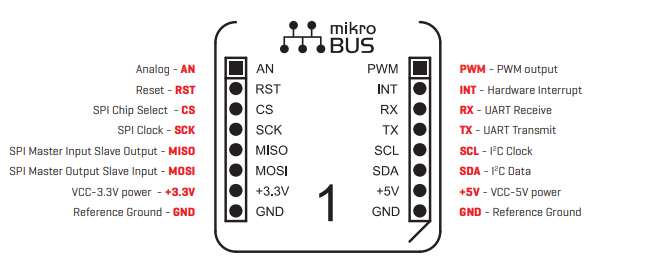
\includegraphics[width=12cm]{Graphics/mikrobus_pinout.png}
    \caption{Specyfikacja wyprowadzeń mikroBUS\texttrademark \cite{mikrobus_specification}}
    \label{img:mikrobus_pinout}
\end{figure}


\section{STM32F103}
Do stworzenia projektu, wybrano procesor STM32F103C8 z rdzeniem ARM\textregistered Cortex\textregistered-M3 \cite{stm_datasheet}. Wybór, podyktowany był przede wszystkim dostępnością, ponieważ układ ten, w obudowach LQFP48 znajdował się w prywatnych zasobach zespołu. Obecnie, na rynku dostępne jest niewiele procesorów, a części elektroniczne są drogie. Z tego powodu, zdecydowano się korzystać z tego, co było dostępne. Nie oznacza to jednak, że procesor ten był pod jakimkolwiek względem ograniczający. Najistotniejszymi z jego cech są:
\begin{itemize}
    \item 2 interfejsy I$^2$C
    \item 3 interfejsy USART
    \item 2 interfejsy SPI
    \item Zasilanie 2.0 - 3.6V
    \item Zewnętrzny zegar 4 - 16MHz
    \item 12-bitowe, wielokanałowe przetworniki A/D
\end{itemize}
Układ, programowany jest przy użyciu interfejsu SWD oraz programatora ST-link. Fakt ten, znacząco ułatwił wykonanie działającego układu. Ze względu na przyjęte założenia i wybrane sensory, wybrany procesor bardzo dobrze wpasowywał się w projekt. Dla wykonania oprogramowania, istotne były również dostarczone przez ST biblioteki oraz oprogramowanie STM32CubeMX, wprowadzające wysoki poziom abstrakcji w tworzeniu oprogramowania. Pozwoliło to uniknąć często czasochłonnego, ręcznego pisania do rejestrów procesora, w celu konfiguracji peryferiów.

\section{STS30}

Sensor STS30-DIS marki Sensirion to cyfrowy, precyzyjny sensor temperatury. Wybrano go jako przykładowy sensor działający po I$^2$C oraz będący bardzo dobrze udokumentowany przez producenta. Oferuje dokładność 0.2 ℃ w zakresie temperatur 0-60 ℃ oraz funkcje takie jak wbudowane ogrzewanie, rejestr statusu, zmienny adres, soft reset po I$^2$C i wiele innych\cite{sts_datasheet}. Wszystkie dane z sensora są weryfikowane CRC-8. Czujnik działa w oparciu o technologię CMOSens\texttrademark, która polega na zależności napięcia progowego tranzystora w technologii CMOS od temperatury. Ta zależność w zakresie działania sensora jest liniowa, co przekłada się na łatwą konwersję napięcia na cyfrową wartość przez przetwornik oraz na konwersję do wartości w stopniach Celsjusza lub Fahrenheita. 
\begin{figure}[H]
    \centering
    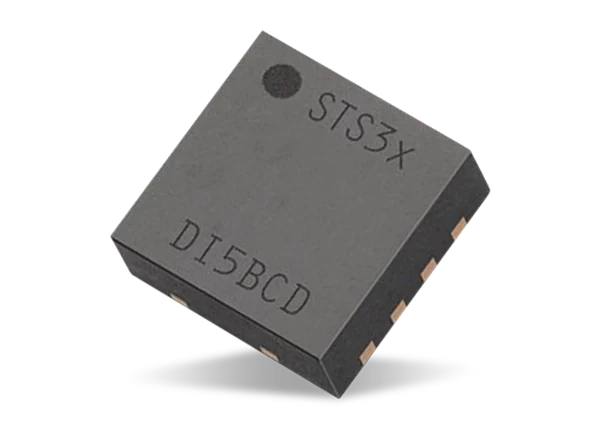
\includegraphics[width=4cm]{Graphics/sts_img.png}
    \caption{Układ STS3x-DIS\cite{sts_mouser}}
    \label{img:sts_mouser}
\end{figure}

\section{BMP280}

Czujnik BMP280 to cyfrowy czujnik ciśnienia atmosferycznego. Pozwala on na pomiary ciśnienia w zakresie 300-1100hPA z dokładnością do jednego hektopaskala. Zasilany napięciem 3.3V, sterowany przy użyciu interfejsu SPI, pobiera mniej niż 2mA prądu. Jest to wyjątkowo popularny układ stosowany nie tylko w amatorskich projektach. Jego dodatkową cechą, jest możliwość pomiaru temperatury z dokładnością 0.01 stopnia celcjusza\cite{bmp_datasheet}.
\newline
BMP280 składa się z piezorezystancyjnego czujnika ciśnienia i dedykowanego układu ASIC, którego zadaniem jest konwersja sygnału analogowego na cyfrowy, jego kompensacja, a następnie transmisja przez interfejs SPI/I2C. Moduł posiada konfigurowalną rozdzielczość pomiaru, dzięki czemu użytkownik może dostosować czujnik pod własne potrzeby, wybierając pomiędzy energooszczędnością a wysoką dokładnością. Dodatkowo układ posiada filtr IIR o konfigurowalnych współczynnikach, którego zadaniem jest eliminacja przypadkowych zaburzeń, jak np. trzaśnięcie drzwiami.
\newline
Rysunek \ref{img:bmp_sampling} przedstawia pełen cykl pomiarowy wykonywany każdorazowo przez moduł. W pierwszej kolejności wykonywany jest pomiar temperatury, ponieważ wykorzystywany jest on do kompensacji zmierzonego później ciśnienia. Następnie w zależności od preferencji użytkownika, nastąpi filtracja, bądź ten krok zostanie pominięty. 

\begin{figure}[H]
    \centering
    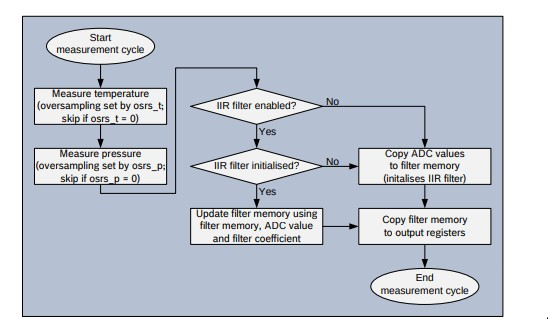
\includegraphics[width=\textwidth, height=\textheight, keepaspectratio]{Graphics/bmp280_sampling.jpg}
    \caption{Cykl pomiarowy BMP280\cite{bmp_datasheet}}
    \label{img:bmp_sampling}
\end{figure}

\begin{figure}[H]
    \centering
    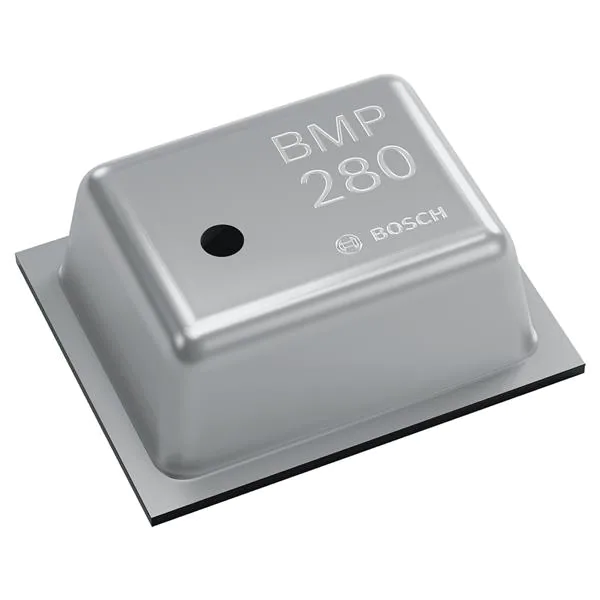
\includegraphics[width=4cm]{Graphics/bmp_img.png}
    \caption{Układ BMP280\cite{bmp_mouser}}
    \label{img:bmp_mouser}
\end{figure}

\section{MQ2}

Czujnik MQ-2 to analogowy czujnik palnych gazów. Zasilany napięciem 5V, pobiera około 150mA prądu. Wynika to ze specyfiki modułu, który w swojej konstrukcji wymaga elementu podgrzewającego. MQ-2 pozwala na wykrywanie LPG, propanu, wodoru i innych gazów wymienionych w dokumentacji układu\cite{mq2_datasheet}.
\newline
Rysunek \ref{img:mq_elements} przedstawia budowę modułu MQ-2. Składa się on z ceramicznej tuby (wykonanej z tritlenku diglinu $Al_2O_3$), warstwy odpowiedzialnej za detekcje gazów (tlenek cyny (IV) $SnO_2$), elektrody pomiarowej oraz wspomnianego już elementu grzewczego. Grzałka zapewnia odpowiednio wysoką temperaturę potrzebną do pracy elementu wykrywającego. Tlenek cyny (IV) zmienia swoją rezystancję w kontakcie z niektórymi gazami. W czystym powietrzu jego przewodność jest niższa i rośnie wraz z koncentracją konkretnych gazów. Zależność tę można wykorzystać tworząc na wyjściu dzielnik napięcia adekwatny do zakresu napieć wykorzystanego mikrokontrolera.
\begin{figure}[H]
    \centering
    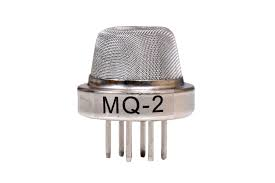
\includegraphics[width=4cm]{Graphics/mq2_img.png}
    \caption{Układ MQ-2\cite{bmp_mouser}}
    \label{img:mq_img}
\end{figure}

\begin{figure}[H]
    \centering
    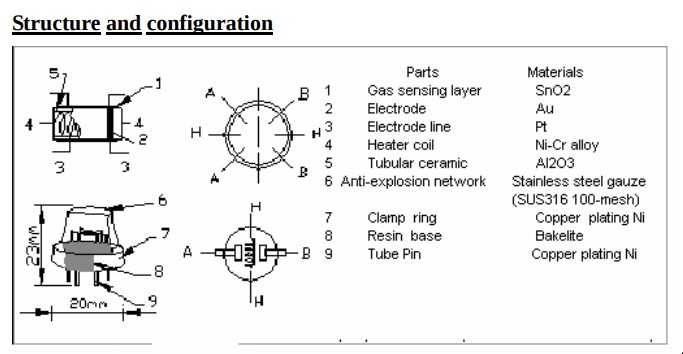
\includegraphics[width=\textwidth, height=\textheight, keepaspectratio]{Graphics/mq_elements.jpg}
    \caption{Konstrukcja MQ-2\cite{mq2_datasheet}}
    \label{img:mq_elements}
\end{figure}

\section{Makefile}
Jednym z założeń, było tworzenie oprogramowania równolegle, na dwóch różnych procesorach. STM32F1 i STM32F4. Procesory te, należąc do zupełnie różnych rodzin, korzystają z innych bibliotek, a do ich konfiguracji niejednokrotnie wymagane są różne kroki. Z tego powodu, w projekcie wykorzystano program \emph{Make}. Pozwala on, na podstawie pliku konfiguracyjnego \emph{makefile}, zdefiniować sposób kompilacji oraz ścieżki bibliotek wykorzystywanych przez kod. Narzędzie to, jest stosunkowo proste w konfiguracji, a jej przykłady są ogólnodostępne w internecie. Dodatkowym argumentem przemawiającym za wykorzystaniem narzędzia, była chęć jego przetestowania w praktyce.

\section{Github}
Github to serwis internetowy pozwalający przechowywać projekty z wykorzystaniem systemu kontroli wersji. Korzysta on z systemu Git opublikowanego na licencji GNU GPL 2 (wolne i otwarte oprogramowanie). System ten, jest obecnie wykorzystywany przez wielu programistów, a jego znajomość często wymagana jest przez pracodawców. Github, poza kontrolą wersji dostarcza wygodne i przejrzyste środowisko w przeglądarce, pozwalające programistom na np. przegląd kodu współpracowników. Fakt ten, został wykorzystany podczas tworzenia projektu. Pozwoliło to nie tylko na poprawienie jakości tworzonego oprogramowania, ale również skonfrontowanie różnych podejść do współpracy nad kodem.
